\documentclass[aspectratio=169]{beamer}
\usepackage{amsmath}
\usepackage{amssymb}
\usepackage{tikz}
\usepackage{xcolor}
\usetikzlibrary{shapes,backgrounds,patterns}

\usepackage{pgfplots}
\pgfplotsset{compat=1.18, legend cell align=left}
\usetikzlibrary{arrows.meta,decorations.pathreplacing,calc,positioning}
\usepackage{booktabs}

% royalblue isn't a base xcolor name, so define it first (this is the default accent)
\definecolor{royalblue}{RGB}{65,105,225}

% ============================================================
%  ACCENT COLOR: change ONE line below to switch the theme
%  Choose one of: royalblue , red , black
% ============================================================
\colorlet{accent}{royalblue}
% \colorlet{accent}{red}
% \colorlet{accent}{black}
% ============================================================

\usetheme{default}
\setbeamercolor{background canvas}{bg=white}
\setbeamercolor{normal text}{fg=black}
\setbeamercolor{structure}{fg=accent}
\setbeamercolor{frametitle}{fg=accent,bg=white}
\setbeamercolor{title}{fg=accent}
\setbeamercolor{section in toc}{fg=black}
\setbeamercolor{block title}{fg=black,bg=gray!10}
\setbeamercolor{block body}{fg=black,bg=gray!5}
\setbeamercolor{block title example}{fg=black,bg=green!10}
\setbeamercolor{block body example}{fg=black,bg=green!5}
\setbeamercolor{block title alerted}{fg=black,bg=red!10}
\setbeamercolor{block body alerted}{fg=black,bg=red!5}

\setbeamertemplate{navigation symbols}{}
\setbeamertemplate{footline}{
    \hfill\makebox[5pt]{%
        \scriptsize\insertframenumber}
    \hspace*{2em}
    \vspace{0.5cm}
}

\newcommand{\cbox}[2]{\colorbox{#1}{\ensuremath{\displaystyle #2}}}

\pgfplotsset{
  miniplot/.style={
    width=4.0cm, height=3.0cm,
    axis lines=middle, xtick=\empty, ytick=\empty,
    samples=120, thick, clip=true
  }
}

\title{Root Finding: Summary}
\subtitle{Bracketing, Newton, and how to combine them}
\author{Sharareh Sayyad}
\institute{Washington State University}
\date{\today}

\begin{document}

\frame{\titlepage}

% ============================================================
% 1. Bisection and false position
% ============================================================
\begin{frame}{Bracketing methods: bisection and false position}
\begin{columns}[c]
\begin{column}{0.47\textwidth}
\small
Start from a \textbf{bracket} $[a,b]$: $f$ continuous, $f(a)$ and $f(b)$ of opposite sign. Pick a point $c$ inside, keep the half with the sign change.
\vspace{0.15cm}
\begin{block}{Bisection: midpoint}
\footnotesize
\[
c = a + \frac{1}{2}\,(b-a)
\]
Uses only the \textbf{sign} of $f$.
\end{block}
\begin{exampleblock}{False position: zero of the secant}
\footnotesize
\[
c = a + \frac{-f(a)}{f(b) - f(a)}\,(b-a)
\]
The weight $\frac12$ is replaced by a fraction in $(0,1)$ set by the \textbf{values} of $f$: often faster, but one endpoint can get stuck.
\end{exampleblock}
\end{column}
\begin{column}{0.5\textwidth}
\centering
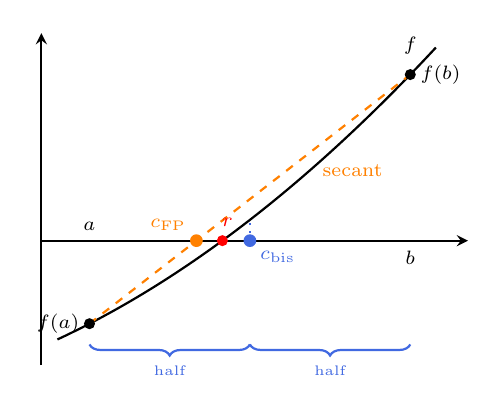
\begin{tikzpicture}
\begin{axis}[width=7.0cm, height=5.8cm, axis lines=middle, xmin=0.85, xmax=2.18, ymin=-1.5, ymax=2.5,
  xtick=\empty, ytick=\empty, samples=80, thick, clip=false]
  \addplot[black, domain=0.9:2.08] {x^2-2};
  \node[font=\scriptsize] at (axis cs:2.0,2.35) {$f$};
  % secant
  \addplot[orange, dashed, domain=1:2] {3*x-4};
  \fill (axis cs:1,-1) circle (2pt) node[left, font=\scriptsize] {$f(a)$};
  \fill (axis cs:2,2) circle (2pt) node[right, font=\scriptsize] {$f(b)$};
  \node[font=\scriptsize, above] at (axis cs:1,0) {$a$};
  \node[font=\scriptsize, below] at (axis cs:2,0) {$b$};
  % bisection midpoint
  \draw[accent, dotted, thick] (axis cs:1.5,0) -- (axis cs:1.5,0.25);
  \fill[accent] (axis cs:1.5,0) circle (2.3pt);
  \node[accent, font=\scriptsize, below right] at (axis cs:1.5,0) {$c_{\text{bis}}$};
  % false position point
  \fill[orange] (axis cs:1.3333,0) circle (2.3pt);
  \node[orange, font=\scriptsize, above left] at (axis cs:1.3333,0) {$c_{\text{FP}}$};
  % root
  \fill[red] (axis cs:1.41421,0) circle (2pt);
  \node[red, font=\scriptsize, above] at (axis cs:1.43,0.05) {$r$};
  % width brace
  \draw[decorate, decoration={brace, amplitude=4pt, mirror}, accent] (axis cs:1,-1.25) -- (axis cs:1.5,-1.25)
     node[midway, below=4pt, font=\tiny] {half};
  \draw[decorate, decoration={brace, amplitude=4pt, mirror}, accent] (axis cs:1.5,-1.25) -- (axis cs:2,-1.25)
     node[midway, below=4pt, font=\tiny] {half};
  \node[orange, font=\scriptsize] at (axis cs:1.82,0.85) {secant};
\end{axis}
\end{tikzpicture}\\[2pt]
\scriptsize Same bracket, two choices of $c$: \textcolor{accent}{midpoint} or \textcolor{orange}{secant zero}.
\end{column}
\end{columns}
\end{frame}

% ============================================================
% 2. When bisection can go wrong
% ============================================================
\begin{frame}{When can bisection go wrong?}
\small Both conditions of the IVT matter (continuity and a sign change). Always \textbf{plot $f$ first}.
\vspace{0.1cm}
\begin{columns}[T]
\begin{column}{0.32\textwidth}
\centering
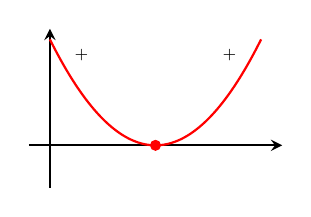
\begin{tikzpicture}
\begin{axis}[miniplot, width=4.8cm, height=3.6cm, xmin=-0.2, xmax=2.2, ymin=-0.4, ymax=1.1]
  \addplot[red, domain=0:2] {(x-1)^2};
  \fill[red] (axis cs:1,0) circle (2pt);
  \node[font=\tiny] at (axis cs:0.3,0.85) {$+$};
  \node[font=\tiny] at (axis cs:1.7,0.85) {$+$};
\end{axis}
\end{tikzpicture}\\[3pt]
\textbf{Root, no sign change}\\[2pt]
\scriptsize $(x-1)^2$ touches the axis but never changes sign: no bracket exists, so the root cannot be found.
\end{column}
\begin{column}{0.32\textwidth}
\centering
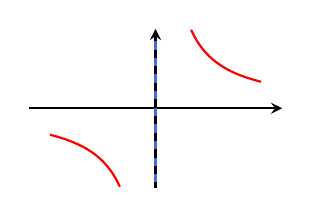
\begin{tikzpicture}
\begin{axis}[miniplot, width=4.8cm, height=3.6cm, xmin=-1.2, xmax=1.2, ymin=-3, ymax=3, restrict y to domain=-3:3]
  \addplot[red, domain=-1:-0.05] {1/x};
  \addplot[red, domain=0.05:1] {1/x};
  \draw[accent, dashed] (axis cs:0,-2.8) -- (axis cs:0,2.8);
\end{axis}
\end{tikzpicture}\\[3pt]
\textbf{Sign change, no root}\\[2pt]
\scriptsize $1/x$ on $[-1,1]$ is not continuous. Bisection ``converges'' to the jump at $x = 0$.
\end{column}
\begin{column}{0.32\textwidth}
\centering
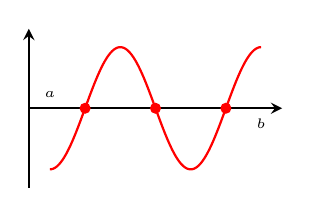
\begin{tikzpicture}
\begin{axis}[miniplot, width=4.8cm, height=3.6cm, xmin=0.2, xmax=3.8, ymin=-1.3, ymax=1.3]
  \addplot[red, domain=0.5:3.5] {-sin(deg(pi*x))};
  \node[font=\tiny, above] at (axis cs:0.5,0) {$a$};
  \node[font=\tiny, below] at (axis cs:3.5,0) {$b$};
  \fill[red] (axis cs:1,0) circle (2pt);
  \fill[red] (axis cs:2,0) circle (2pt);
  \fill[red] (axis cs:3,0) circle (2pt);
\end{axis}
\end{tikzpicture}\\[3pt]
\textbf{Several roots}\\[2pt]
\scriptsize Still a sign change, but you get \emph{one} root, and which one depends on the bracket.
\end{column}
\end{columns}
\vspace{0.15cm}
\begin{alertblock}{Also watch for}
\scriptsize
\textbf{Tolerance below machine precision} ($\text{tol} < 10^{-16}|r|$): the midpoint equals $a$ or $b$ and the loop never ends, so always cap with \texttt{maxit}. \quad
\textbf{False position:} a stuck endpoint can make it much \emph{slower} than bisection.
\end{alertblock}
\end{frame}

% ============================================================
% 3. Guaranteed, linear, steps from tolerance
% ============================================================
\begin{frame}{Bisection: guaranteed, linear, and predictable}
\begin{columns}[T]
\begin{column}{0.47\textwidth}
\small
\begin{itemize}
  \item \textbf{Guaranteed}: the bracket always contains a root.
  \item \textbf{Linear}, $\rho = \tfrac12$: the bound halves every step.
\end{itemize}
\begin{block}{Steps from the tolerance}
\footnotesize
\vspace{-0.15cm}
\[
|c_n - r| \le \frac{b-a}{2^{\,n}} \le \text{tol}
\;\Longleftrightarrow\;
\cbox{accent!12}{n \ge \log_2\frac{b-a}{\text{tol}}}
\]
$r$ is in the bracket and $c_n$ is its midpoint: $|c_n - r| \le$ half its width. Known \textbf{before} we start.
\end{block}
\centering
\scriptsize
\setlength{\tabcolsep}{5pt}
\begin{tabular}{lccc}
\toprule
$[a,b] = [1,2]$, tol & $10^{-3}$ & $10^{-6}$ & $10^{-12}$ \\
\midrule
steps $n$ & 10 & 20 & 40 \\
\bottomrule
\end{tabular}\\[3pt]
\raggedright
Cost $= O(\log(1/\text{tol}))$: $10\times$ accuracy $\approx 3.3$ more steps.
\end{column}
\begin{column}{0.5\textwidth}
\centering
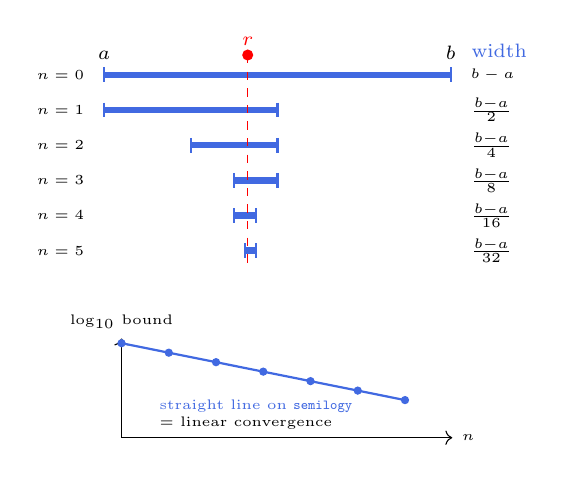
\begin{tikzpicture}[x=4.4cm, y=0.72cm]
  % root position for x^2 - 2 on [1,2]
  \def\r{0.41421}
  \foreach \a/\b/\n/\w in {0/1/0/{b-a}, 0/0.5/1/{\tfrac{b-a}{2}}, 0.25/0.5/2/{\tfrac{b-a}{4}}, 0.375/0.5/3/{\tfrac{b-a}{8}}, 0.375/0.4375/4/{\tfrac{b-a}{16}}, 0.40625/0.4375/5/{\tfrac{b-a}{32}}} {
    \draw[accent, line width=2.4pt] (\a,-0.62*\n) -- (\b,-0.62*\n);
    \draw[accent, thick] (\a,-0.62*\n+0.13) -- (\a,-0.62*\n-0.13);
    \draw[accent, thick] (\b,-0.62*\n+0.13) -- (\b,-0.62*\n-0.13);
    \node[font=\tiny, left] at (-0.03,-0.62*\n) {$n=\n$};
    \node[font=\tiny, right] at (1.03,-0.62*\n) {$\w$};
  }
  \draw[red, dashed, thin] (\r,0.35) -- (\r,-3.4);
  \fill[red] (\r,0.35) circle (2pt) node[above, font=\scriptsize] {$r$};
  \node[font=\scriptsize, above] at (0,0.1) {$a$};
  \node[font=\scriptsize, above] at (1,0.1) {$b$};
  \node[font=\scriptsize, accent] at (1.14,0.42) {width};
  % error-bound staircase
  \begin{scope}[shift={(0.05,-6.4)}, x=0.6cm, y=0.2cm]
    \draw[->] (0,0) -- (7,0) node[right, font=\tiny] {$n$};
    \draw[->] (0,0) -- (0,6.3) node[above, font=\tiny] {$\log_{10}$ bound};
    \draw[accent, thick] (0,6) -- (6,6-6*0.301*2);
    \foreach \k in {0,...,6} \fill[accent] (\k,{6-\k*0.301*2}) circle (1.5pt);
    \node[font=\tiny, accent, anchor=west] at (0.6,2.0) {straight line on \texttt{semilogy}};
    \node[font=\tiny, anchor=west] at (0.6,0.9) {$=$ linear convergence};
  \end{scope}
\end{tikzpicture}
\end{column}
\end{columns}
\end{frame}

% ============================================================
% 4. Newton: local and quadratic
% ============================================================
\begin{frame}{Newton's method: fast, but only local}
\begin{columns}[c]
\begin{column}{0.47\textwidth}
\small
Follow the \textbf{tangent line} at $x_n$ to the axis:
\[
\cbox{accent!12}{x_{n+1} = x_n - \frac{f(x_n)}{f'(x_n)}}
\]
\vspace{-0.2cm}
\begin{block}{Quadratic convergence}
\footnotesize
$e_{n+1} \approx \dfrac{f''(r)}{2f'(r)}\,e_n^2$: correct digits \textbf{double} each step.\\[2pt]
If $|e_n| \approx 10^{-k}$, then $|e_{n+1}| \approx C\cdot 10^{-2k}$.
\end{block}
\begin{alertblock}{Local: no guarantee}
\footnotesize
Converges only if $x_0$ is \textbf{close enough} ($|x_0 - r| < \delta$, with $\delta$ unknown) and $f'(r) \neq 0$. No bracket, no error bound in advance.
\end{alertblock}
\end{column}
\begin{column}{0.5\textwidth}
\centering
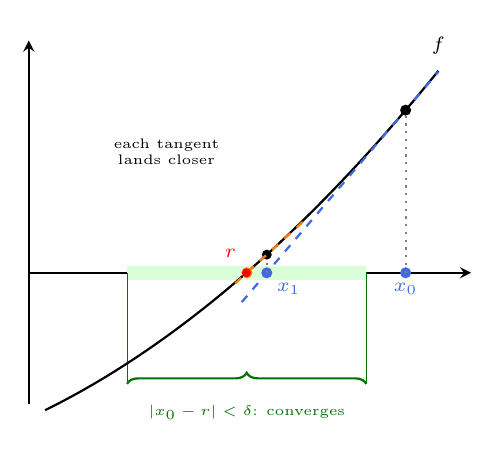
\begin{tikzpicture}
\begin{axis}[width=7.2cm, height=6.2cm, axis lines=middle, xmin=0.75, xmax=2.1, ymin=-1.3, ymax=2.3,
  xtick=\empty, ytick=\empty, samples=80, thick, clip=false]
  % basin of attraction (schematic)
  \fill[green!15] (axis cs:1.05,-0.07) rectangle (axis cs:1.78,0.07);
  \draw[decorate, decoration={brace, amplitude=4pt}, green!45!black] (axis cs:1.05,-1.1) -- (axis cs:1.78,-1.1)
    node[midway, below=4pt, font=\tiny, green!45!black] {$|x_0 - r| < \delta$: converges};
  \draw[green!45!black, thin] (axis cs:1.05,-1.1) -- (axis cs:1.05,0);
  \draw[green!45!black, thin] (axis cs:1.78,-1.1) -- (axis cs:1.78,0);
  \addplot[black, domain=0.8:2.0] {x^2-2};
  \node[font=\scriptsize] at (axis cs:2.0,2.25) {$f$};
  % tangent at x0 = 1.9 (schematic, start right)
  \addplot[accent, dashed, domain=1.4:2.0] {1.61+3.8*(x-1.9)};
  \fill (axis cs:1.9,1.61) circle (2pt);
  \fill[accent] (axis cs:1.9,0) circle (2pt) node[below, font=\scriptsize] {$x_0$};
  \draw[gray, dotted] (axis cs:1.9,0) -- (axis cs:1.9,1.61);
  \fill[accent] (axis cs:1.47632,0) circle (2pt) node[below right, font=\scriptsize, accent] {$x_1$};
  \draw[gray, dotted] (axis cs:1.47632,0) -- (axis cs:1.47632,0.17952);
  \fill (axis cs:1.47632,0.17952) circle (1.8pt);
  \addplot[orange, dashed, domain=1.38:1.6] {0.17952+2.95264*(x-1.47632)};
  \fill[orange] (axis cs:1.41552,0) circle (2pt);
  % root
  \fill[red] (axis cs:1.41421,0) circle (1.6pt);
  \node[red, font=\scriptsize, above left] at (axis cs:1.41421,0.05) {$r$};
  \node[font=\tiny, align=center] at (axis cs:1.17,1.2) {each tangent\\lands closer};
\end{axis}
\end{tikzpicture}
\end{column}
\end{columns}
\end{frame}

% ============================================================
% 5. Finite-difference Newton and secant
% ============================================================
\begin{frame}{Newton without $f'$: finite differences and secant}
\small Newton only needs \textbf{a slope} at $x_n$. Choose the variation by what you have:
\vspace{0.15cm}
\begin{columns}[T]
\begin{column}{0.49\textwidth}
\begin{block}{$f$ is a function, but $f'$ is not given}
\footnotesize
\textbf{Finite-difference Newton:} evaluate $f$ at a nearby point
\[
f'(x_n) \approx \frac{f(x_n + h) - f(x_n)}{h},\qquad h \approx 10^{-8}|x_n|
\]
Each step costs \textbf{2 evaluations of $f$}: $f(x_n)$ and $f(x_n+h)$. Nearly quadratic. $h$ too big: slope error; too small: rounding.
\end{block}
\centering
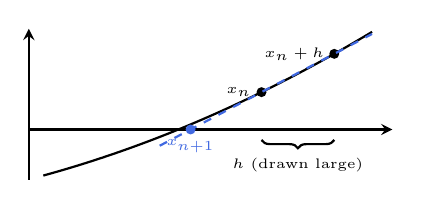
\begin{tikzpicture}
\begin{axis}[width=6.2cm, height=3.5cm, axis lines=middle, xmin=0.9, xmax=2.15, ymin=-1.2, ymax=2.4,
  xtick=\empty, ytick=\empty, samples=80, thick, clip=false]
  \addplot[black, domain=0.95:2.08] {x^2-2};
  \fill (axis cs:1.7,0.89) circle (1.8pt) node[left, font=\tiny] {$x_n$};
  \fill (axis cs:1.95,1.8025) circle (1.8pt) node[left, font=\tiny] {$x_n + h$};
  \addplot[accent, dashed, domain=1.35:2.08] {0.89+3.65*(x-1.7)};
  \fill[accent] (axis cs:1.4562,0) circle (1.8pt) node[below, font=\tiny, accent] {$x_{n+1}$};
  \draw[decorate, decoration={brace, amplitude=3pt, mirror}] (axis cs:1.7,-0.25) -- (axis cs:1.95,-0.25)
    node[midway, below=3pt, font=\tiny] {$h$ (drawn large)};
\end{axis}
\end{tikzpicture}
\end{column}
\begin{column}{0.49\textwidth}
\begin{exampleblock}{Only a handful of points $(x_k, f_k)$}
\footnotesize
\textbf{Secant method:} slope through the \textbf{two newest} points
\[
x_{n+1} = x_n - f_n\,\frac{x_n - x_{n-1}}{f_n - f_{n-1}}
\]
No $f'$, no bracket. Each step costs \textbf{1 evaluation of $f$}, at the new point $x_{n+1}$; $f_{n-1}$ is reused. Order $\approx 1.618$.
\end{exampleblock}
\centering
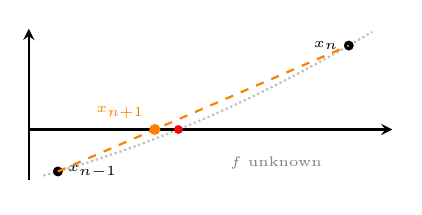
\begin{tikzpicture}
\begin{axis}[width=6.2cm, height=3.5cm, axis lines=middle, xmin=0.9, xmax=2.15, ymin=-1.2, ymax=2.4,
  xtick=\empty, ytick=\empty, samples=80, thick, clip=false]
  \addplot[gray!50, densely dotted, domain=0.95:2.08] {x^2-2};
  \node[gray, font=\tiny] at (axis cs:1.75,-0.8) {$f$ unknown};
  \fill (axis cs:1,-1) circle (1.8pt) node[right, font=\tiny] {$x_{n-1}$};
  \fill (axis cs:2,2) circle (1.8pt) node[left, font=\tiny] {$x_n$};
  \addplot[orange, dashed, domain=1:2] {3*x-4};
  \fill[orange] (axis cs:1.3333,0) circle (2pt) node[above left, font=\tiny, orange] {$x_{n+1}$};
  \fill[red] (axis cs:1.41421,0) circle (1.6pt);
\end{axis}
\end{tikzpicture}
\end{column}
\end{columns}
\end{frame}

% ============================================================
% 6. When Newton (and variations) can go wrong
% ============================================================
\begin{frame}{When can Newton (or secant) go wrong?}
\small Only \emph{local} information: far from the root, the tangent (or secant) can point anywhere.
\vspace{0.2cm}
\begin{columns}[T]
\begin{column}{0.32\textwidth}
\centering
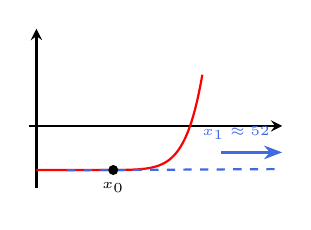
\begin{tikzpicture}
\begin{axis}[miniplot, width=4.8cm, height=3.6cm, xmin=-0.05, xmax=1.6, ymin=-1.4, ymax=2.2, clip=false]
  \addplot[red, domain=0:1.08, samples=150] {x^10-1};
  \addplot[accent, dashed, domain=0.2:1.6] {-0.99902+0.01953*(x-0.5)};
  \fill (axis cs:0.5,-0.999) circle (1.8pt);
  \node[font=\tiny, below] at (axis cs:0.5,-1.05) {$x_0$};
  \draw[-{Stealth}, accent] (axis cs:1.2,-0.6) -- (axis cs:1.6,-0.6);
  \node[accent, font=\tiny, above] at (axis cs:1.3,-0.55) {$x_1 \approx 52$};
\end{axis}
\end{tikzpicture}\\[2pt]
\textbf{\footnotesize Flat tangent}\\[1pt]
\scriptsize $f'(x_n) \approx 0$: huge overshoot. $f'(x_n) = 0$: step undefined.
\end{column}
\begin{column}{0.32\textwidth}
\centering
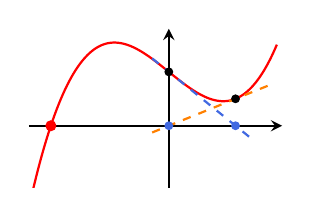
\begin{tikzpicture}
\begin{axis}[miniplot, width=4.8cm, height=3.6cm, xmin=-2.1, xmax=1.7, ymin=-2.3, ymax=3.6]
  \addplot[red, domain=-2.05:1.62] {x^3-2*x+2};
  \addplot[accent, dashed, domain=-0.25:1.25] {2-2*x};
  \addplot[orange, dashed, domain=-0.25:1.5] {x};
  \fill (axis cs:0,2) circle (1.6pt);
  \fill (axis cs:1,1) circle (1.6pt);
  \fill[accent] (axis cs:0,0) circle (1.6pt);
  \fill[accent] (axis cs:1,0) circle (1.6pt);
  \fill[red] (axis cs:-1.769,0) circle (2pt);
\end{axis}
\end{tikzpicture}\\[2pt]
\textbf{\footnotesize Cycling}\\[1pt]
\scriptsize $x^3 - 2x + 2$ from $x_0 = 0$: $0, 1, 0, 1, \ldots$ forever.
\end{column}
\begin{column}{0.32\textwidth}
\centering
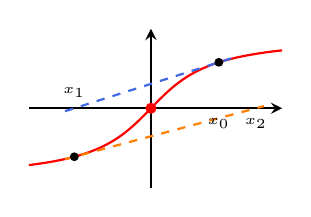
\begin{tikzpicture}
\begin{axis}[miniplot, width=4.8cm, height=3.6cm, xmin=-2.7, xmax=2.9, ymin=-1.7, ymax=1.7]
  \addplot[red, domain=-2.7:2.9] {rad(atan(x))};
  \addplot[accent, dashed, domain=-1.9:1.8] {0.98279+0.30769*(x-1.5)};
  \addplot[orange, dashed, domain=-1.9:2.5] {-1.03755+0.25840*(x+1.69408)};
  \fill (axis cs:1.5,0.98279) circle (1.6pt);
  \fill (axis cs:-1.69408,-1.03755) circle (1.6pt);
  \node[font=\tiny, below] at (axis cs:1.5,0) {$x_0$};
  \node[font=\tiny, above] at (axis cs:-1.69408,0) {$x_1$};
  \node[font=\tiny, below] at (axis cs:2.32,0) {$x_2$};
  \fill[red] (axis cs:0,0) circle (2pt);
\end{axis}
\end{tikzpicture}\\[2pt]
\textbf{\footnotesize Divergence}\\[1pt]
\scriptsize $\arctan x$ from $x_0 = 1.5$: $-1.69, 2.32, -5.11, \ldots$
\end{column}
\end{columns}
\vspace{0.25cm}
\begin{alertblock}{Defences}
\scriptsize Start close (plot $f$ first) $\cdot$ cap with \texttt{maxit} and \textbf{raise} if reached $\cdot$ a small step is not a root: also check $|f(x)|$ $\cdot$ secant: $f_n = f_{n-1}$ gives division by zero.
\end{alertblock}
\end{frame}

% ============================================================
% 7. Bisection + Newton
% ============================================================
\begin{frame}{Best of both: bisection + Newton (safeguarded Newton)}
\begin{columns}[c]
\begin{column}{0.44\textwidth}
\small
Keep a bracket $[a,b]$ at all times. Each step:
\vspace{0.15cm}

\centering
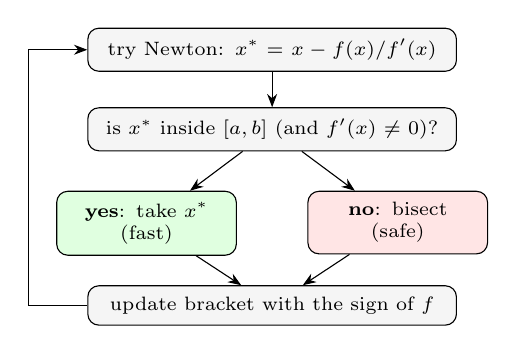
\begin{tikzpicture}[node distance=0.45cm, font=\scriptsize,
  box/.style={draw, rounded corners, fill=gray!8, align=center, inner sep=4pt, text width=4.4cm},
  ok/.style={draw, rounded corners, fill=green!12, align=center, inner sep=4pt, text width=2.0cm},
  no/.style={draw, rounded corners, fill=red!10, align=center, inner sep=4pt, text width=2.0cm}]
  \node[box] (n) {try Newton: $x^* = x - f(x)/f'(x)$};
  \node[box, below=of n] (q) {is $x^*$ inside $[a,b]$ (and $f'(x) \ne 0$)?};
  \node[ok, below left=0.5cm and -1.9cm of q] (y) {\textbf{yes}: take $x^*$\\(fast)};
  \node[no, below right=0.5cm and -1.9cm of q] (z) {\textbf{no}: bisect\\(safe)};
  \node[box, below=1.7cm of q] (u) {update bracket with the sign of $f$};
  \draw[-{Stealth}] (n) -- (q);
  \draw[-{Stealth}] (q) -- (y);
  \draw[-{Stealth}] (q) -- (z);
  \draw[-{Stealth}] (y) -- (u);
  \draw[-{Stealth}] (z) -- (u);
  \draw[-{Stealth}] (u.west) -- ++(-0.75,0) |- (n.west);
\end{tikzpicture}

\vspace{0.15cm}
\raggedright
\scriptsize
\textbf{Guaranteed} like bisection; \textbf{quadratic} near the root like Newton.
\end{column}
\begin{column}{0.54\textwidth}
\centering
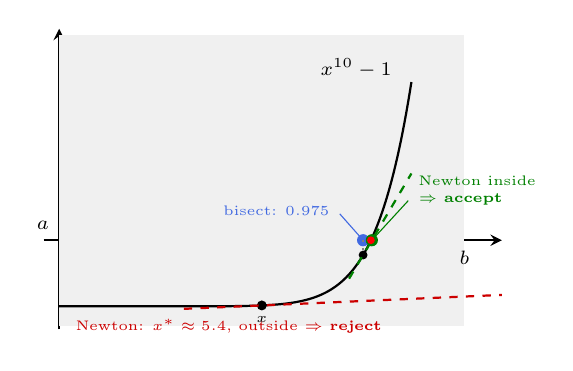
\begin{tikzpicture}
\begin{axis}[width=7.4cm, height=5.4cm, axis lines=middle, xmin=-0.05, xmax=1.42, ymin=-1.35, ymax=3.2,
  xtick=\empty, ytick=\empty, samples=200, thick, clip=false]
  \fill[gray!12] (axis cs:0,-1.3) rectangle (axis cs:1.3,3.1);
  \addplot[black, domain=0:1.13] {x^10-1};
  \node[font=\scriptsize, left] at (axis cs:1.1,2.6) {$x^{10}-1$};
  \node[font=\scriptsize, above left] at (axis cs:0,0) {$a$};
  \node[font=\scriptsize, below] at (axis cs:1.3,0) {$b$};
  % step 1: Newton from x = 0.65 shoots outside
  \fill (axis cs:0.65,-0.98654) circle (1.8pt);
  \node[font=\tiny, below] at (axis cs:0.65,-1.0) {$x$};
  \addplot[red!80!black, dashed, domain=0.4:1.42] {-0.98654+0.20711*(x-0.65)};
  \node[red!80!black, font=\tiny, anchor=west] at (axis cs:0.02,-1.3) {Newton: $x^* \approx 5.4$, outside $\Rightarrow$ \textbf{reject}};
  % bisection point
  \fill[accent] (axis cs:0.975,0) circle (2.2pt);
  \node[accent, font=\tiny, anchor=east] at (axis cs:0.9,0.45) {bisect: $0.975$};
  \draw[accent, thin] (axis cs:0.9,0.4) -- (axis cs:0.975,0);
  % step 2: Newton from 0.975 lands inside
  \fill (axis cs:0.975,-0.22357) circle (1.6pt);
  \draw[gray, dotted] (axis cs:0.975,0) -- (axis cs:0.975,-0.22357);
  \addplot[green!50!black, dashed, domain=0.93:1.13] {-0.22357+7.9599*(x-0.975)};
  \fill[green!50!black] (axis cs:1.0031,0) circle (2.2pt);
  \node[green!50!black, font=\tiny, align=left, anchor=west] at (axis cs:1.12,0.75) {Newton inside\\$\Rightarrow$ \textbf{accept}};
  \draw[green!50!black, thin] (axis cs:1.0031,0) -- (axis cs:1.12,0.6);
  \fill[red] (axis cs:1,0) circle (1.4pt);
\end{axis}
\end{tikzpicture}\\[3pt]
\scriptsize
\tiny
\setlength{\tabcolsep}{3pt}
\begin{tabular}{lccccc}
\toprule
$x^{10}-1$, $[0,1.3]$ & bisect. & false pos. & Illinois & Newton & safeguarded \\
\midrule
steps to $10^{-6}$ & 20 & 61 & 13 & 21 & \cbox{green!15}{4} \\
\bottomrule
\end{tabular}
\end{column}
\end{columns}
\end{frame}

\end{document}
